\documentclass[xcolor=dvipsnames]{beamer}
\usetheme{nelle}
\usepackage{natbib}                 % Fancy bibliography.
\usepackage{url}                    % Allow printing of URLs.
\usepackage{outlines}
\usepackage{enumitem}
\usepackage{multicol}
\usepackage{dsfont}
\usepackage{amsmath}
\usepackage{epstopdf}
\usepackage{listings}
\usepackage{enumerate}
\usepackage{tabularx}
\usepackage[normalem]{ulem}

\usepackage{color}
\setbeamerfont{caption}{size=\scriptsize}
\setbeamertemplate{navigation symbols}{}
\setbeamertemplate{footline}[frame number]{}
\newcommand{\heading}[1]{\multicolumn{1}{c}{#1}}

\def\newblock{\hskip .11em plus .33em minus .07em}
\usepackage{color}

\definecolor{mygreen}{rgb}{0,0.6,0}
\definecolor{mygray}{rgb}{0.5,0.5,0.5}
\definecolor{mymauve}{rgb}{0.58,0,0.82}

\lstset{ %
  backgroundcolor=\color{white},   % choose the background color; you must add \usepackage{color} or \usepackage{xcolor}; should come as last argument
  basicstyle=\scriptsize,        % the size of the fonts that are used for the code
  breakatwhitespace=false,         % sets if automatic breaks should only happen at whitespace
  breaklines=true,                 % sets automatic line breaking
  captionpos=b,                    % sets the caption-position to bottom
  commentstyle=\color{mygreen},    % comment style
  deletekeywords={...},            % if you want to delete keywords from the given language
  escapeinside={\%*}{*)},          % if you want to add LaTeX within your code
  extendedchars=true,              % lets you use non-ASCII characters; for 8-bits encodings only, does not work with UTF-8
  keepspaces=true,                 % keeps spaces in text, useful for keeping indentation of code (possibly needs columns=flexible)
  keywordstyle=\color{blue},       % keyword style
  language=Python,                 % the language of the code
  morekeywords={*,...},            % if you want to add more keywords to the set
  rulecolor=\color{black},         % if not set, the frame-color may be changed on line-breaks within not-black text (e.g. comments (green here))
  showspaces=false,                % show spaces everywhere adding particular underscores; it overrides 'showstringspaces'
  showstringspaces=false,          % underline spaces within strings only
  showtabs=false,                  % show tabs within strings adding particular underscores
  stringstyle=\color{mymauve},     % string literal style
  tabsize=2,                     % sets default tabsize to 2 spaces
  title=\lstname                   % show the filename of files included with \lstinputlisting; also try caption instead of title
}

\newcommand{\todo}[1]{\textbf{[TODO: #1]}}
\newcommand{\fixme}[1]{\textbf{[FIXME: #1]}}


\title{\textbf{A Scientific approach to understanding open-source communities}}

\author[Varoquaux Nelle]{
Nelle Varoquaux}


\date{December, 3rd}
\institute{Mines ParisTech, Institut Curie, INSERM}
\begin{document}
\begin{frame}[t, noframenumbering]
  \maketitle

\end{frame}

\setcounter{framenumber}{0}


\begin{frame}
\frametitle{}

\begin{center}
\includegraphics[width=0.8\linewidth]{figures/Open-Source-Word-Cloud.jpg}
\end{center}
\end{frame}

\begin{frame}
{\Large \bf Most opensource software are not successful}
\begin{itemize}[label={$\bullet$}]
\item only 1/6 project is successfull
\item 46\% are abandonned before the first release.
\item 37\% after the first release
\item 17\% are successful
\end{itemize}
\begin{flushright}
% FIXME
{\scriptsize}
\end{flushright}
\end{frame}

\begin{frame}
\hspace{-3em}
\begin{columns}
\begin{column}{0.6\linewidth}
{\Large \bf ``An opensource software is only as successful as its community''}
\end{column}
\begin{column}{0.4\linewidth}
\end{column}
\end{columns}
\begin{flushright}
\includegraphics[width=0.7\linewidth]{images/community.png}
\end{flushright}
\end{frame}

\begin{frame}
\frametitle{}
{\Large \bf So why is that?}
\end{frame}

\begin{frame}
\frametitle{Several people, several opinions\dots}
\begin{columns}
\begin{column}{0.3\linewidth}
\includegraphics[width=0.9\linewidth]{figures/pieter_hintjens.jpg}
\end{column}

\begin{column}{0.3\linewidth}
\includegraphics[width=0.9\linewidth]{figures/gael_varoquaux.jpg}
\end{column}

\begin{column}{0.3\linewidth}
\includegraphics[width=0.9\linewidth]{figures/yuvi.png}
\end{column}

\end{columns}
\end{frame}

\begin{frame}
\frametitle{}
{\Large \bf A scientific approach to understanding open source
communities?}
\end{frame}

\begin{frame}
\frametitle{Why is a scientific approach necessary?}
\begin{columns}
\begin{column}{0.6\linewidth}
{\Large \bf ``Which claims are verifiable, and which are merely wishful
thinking?''}
\end{column}
\begin{column}{0.4\linewidth}
\includegraphics[width=0.9\linewidth]{figures/making_software.jpg}
\end{column}
\end{columns}
\end{frame}

\begin{frame}
\frametitle{3 examples of unverifiable or wrong claims}
\begin{columns}
\begin{column}{0.5\linewidth}
{\Large \bf The best way to treat breast cancer}
\end{column}
\begin{column}{0.5\linewidth}
\includegraphics[width=0.9\linewidth]{figures/breast-cancer-dp.jpg}
\end{column}
\end{columns}
\end{frame}

\begin{frame}
\frametitle{3 examples of unverifiable or wrong claims}
\begin{columns}
\begin{column}{0.5\linewidth}
{\Large \bf Preventing infection during brain surgery}
\end{column}
\begin{column}{0.5\linewidth}
\includegraphics[width=0.9\linewidth]{figures/brain-icon-03.png}
\end{column}
\end{columns}
\end{frame}

\begin{frame}
\frametitle{3 examples of unverifiable or wrong claims}
\begin{columns}
\begin{column}{0.5\linewidth}
{\Large \bf Does test-driven development really work?}
\end{column}
\begin{column}{0.5\linewidth}
\includegraphics[width=0.9\linewidth]{figures/tdd.png}
\end{column}
\end{columns}
\end{frame}

\begin{frame}
\frametitle{}
{\Large \bf So how do we study open-source communities using scientific
approaches?}
\end{frame}

\begin{frame}
\frametitle{The Berkeley Institute for Data Science}
\begin{center}
\only<1>{\includegraphics[width=0.4\linewidth]{images/bids.png}}
\only<2>{
\begin{columns}
\begin{column}{0.3\linewidth}
\includegraphics[width=0.9\linewidth]{images/charlotte_2.jpg}
\end{column}
\begin{column}{0.3\linewidth}
\includegraphics[width=0.9\linewidth]{images/stuart.png}
\end{column}
\begin{column}{0.3\linewidth}
\includegraphics[width=0.9\linewidth]{images/chris_1.png}
\end{column}
\end{columns}
}
\end{center}
\end{frame}

\begin{frame}
\frametitle{The Ethnographer's approach}

{\em
``Ethnography is an approach to understanding cultural life that is founded
not just on witnessing but on participation, with the goal of
understanding
not simply what people are doing, but how they experience what they
do.''}
\vspace{3em}
\begin{flushright}
--Paul Dourish, Reading and Interpreting Ethnography
\end{flushright}
\end{frame}

\usebackgroundtemplate{%             declare it
\tikz[overlay,remember picture] \node[opacity=1, at=(current page.center)] {
  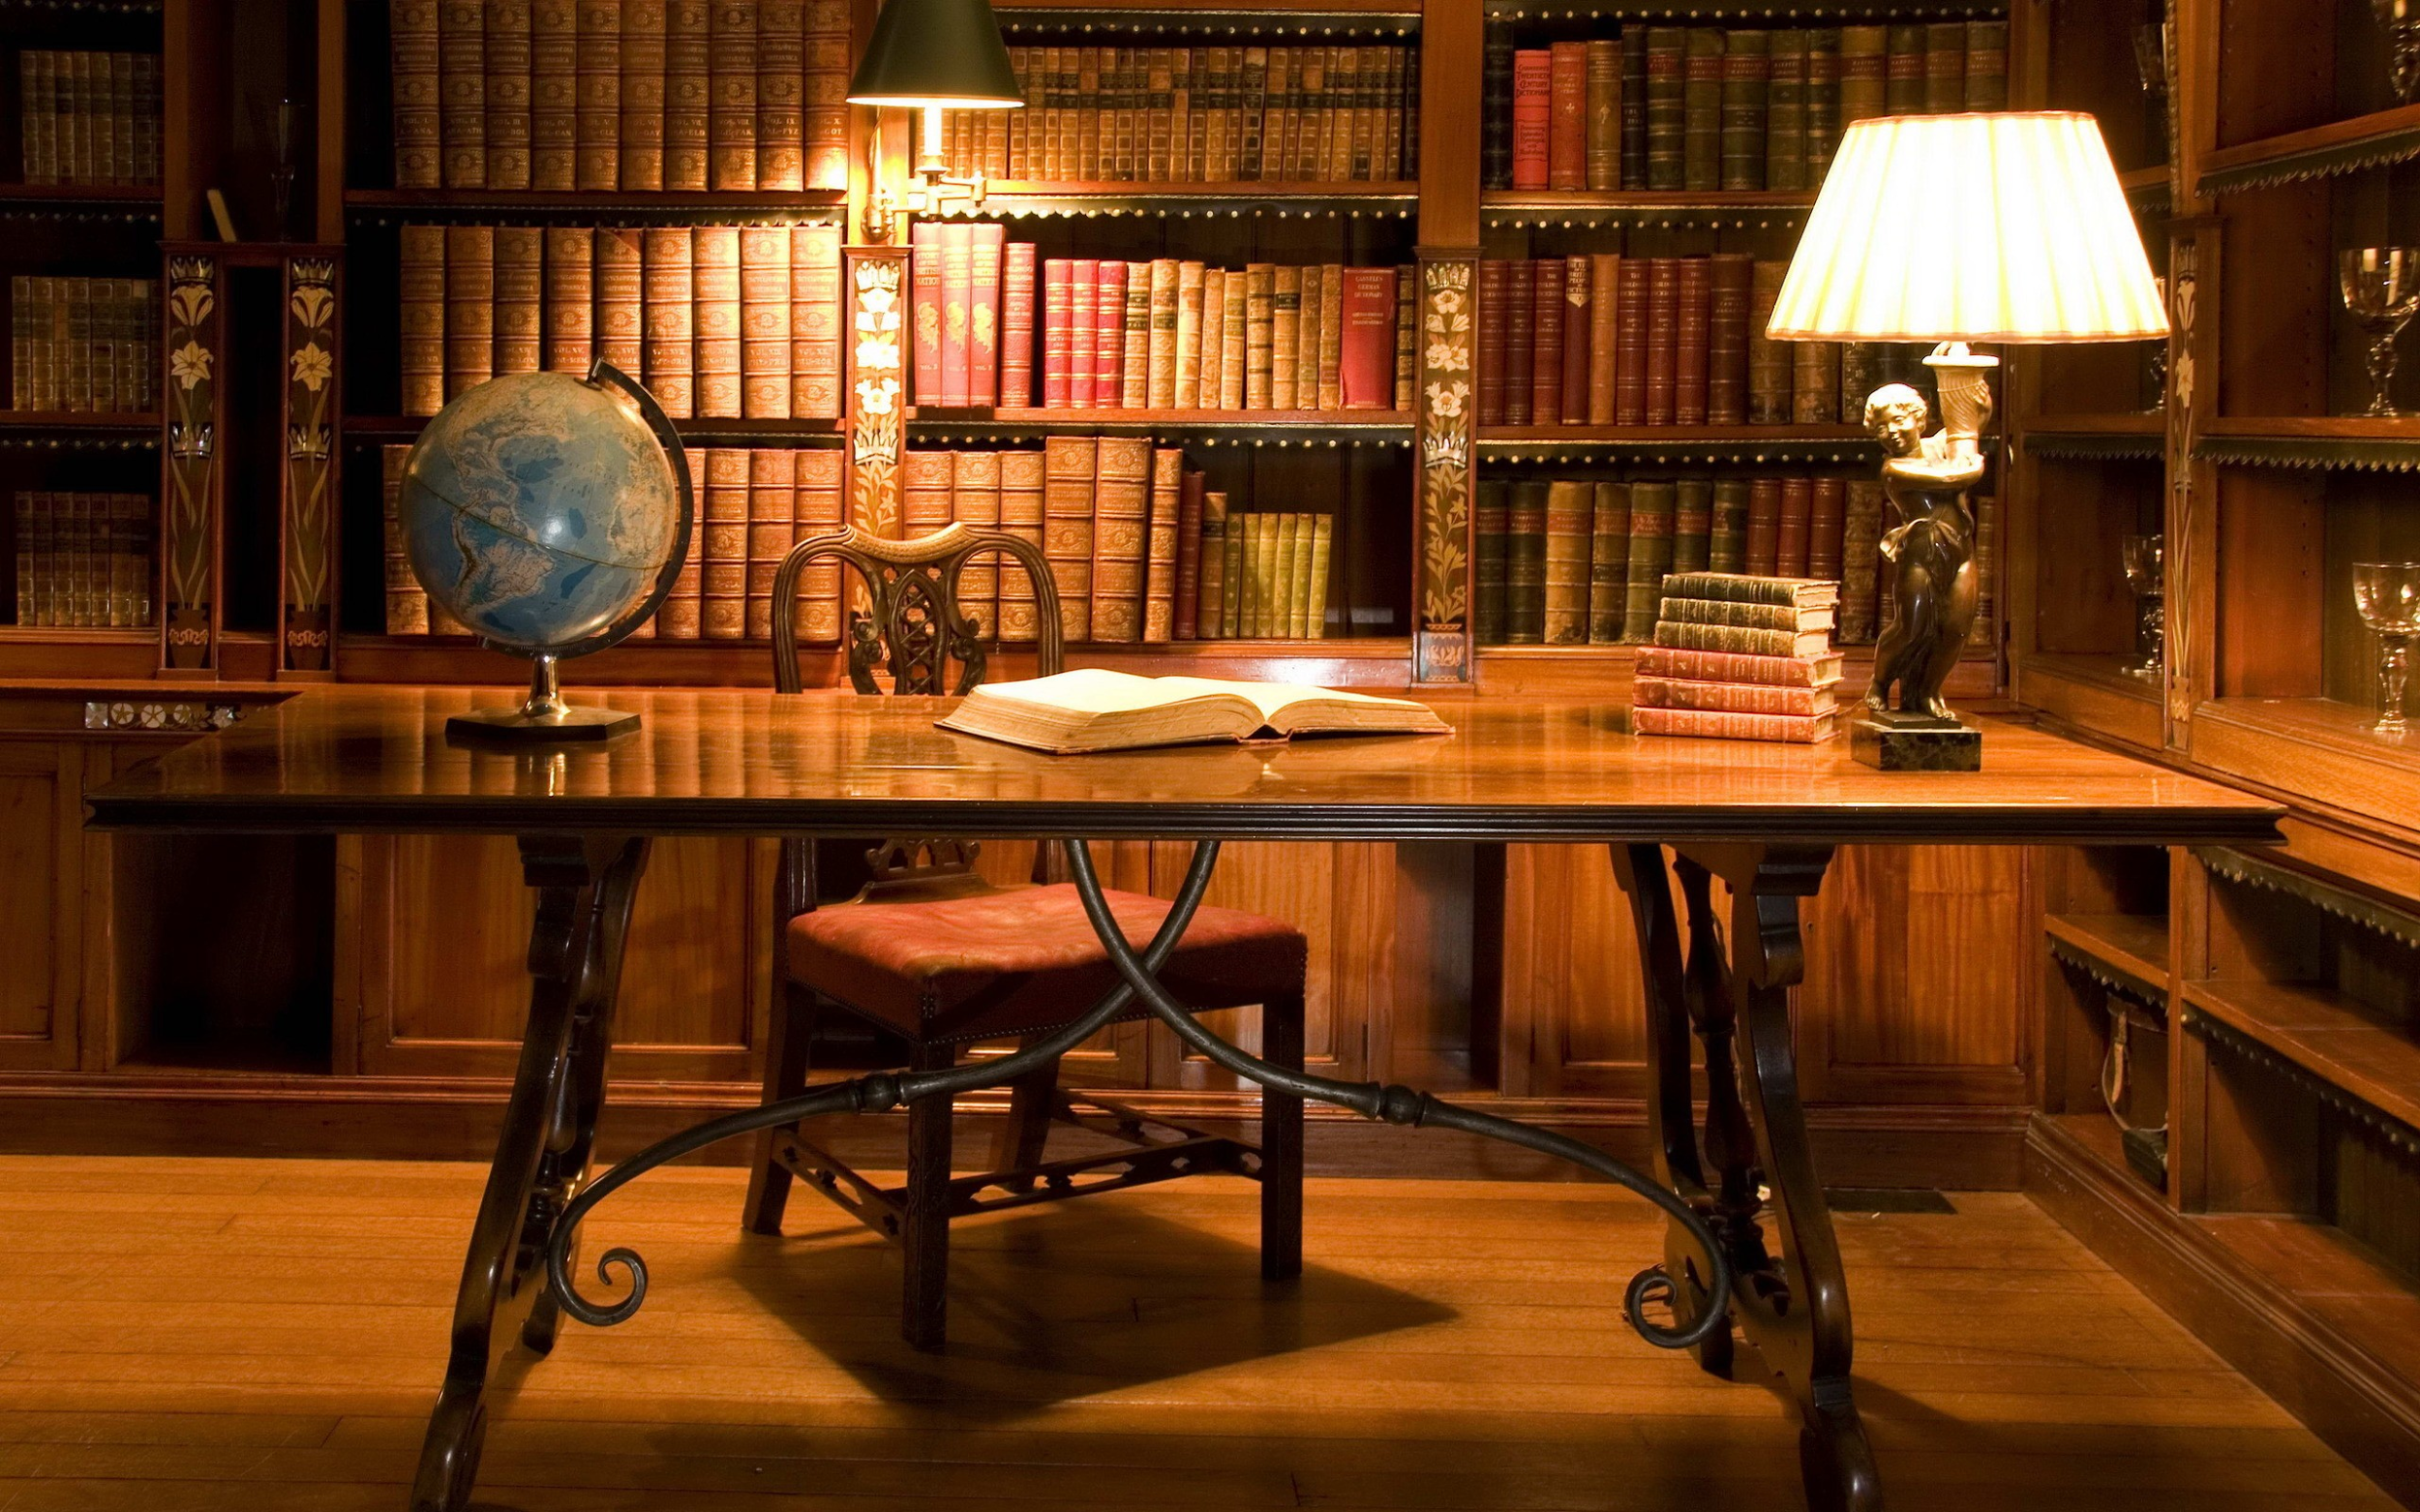
\includegraphics[height=\paperheight,width=\paperwidth]{figures/ethnography.png}};
}

\begin{frame}
\end{frame}
\usebackgroundtemplate{ }  

\begin{frame}
\frametitle{Ethnography methods}
\begin{columns}
\begin{column}{0.5\linewidth}
\begin{itemize}[label={$\bullet$}]
\item Interviews (un/semi-structured)
\item Focus groups
\item Field observation
\item Participant-observation
\end{itemize}
\end{column}
\begin{column}{0.5\linewidth}
\begin{itemize}[label={$\bullet$}]
\item Case studies
\item Oral histories
\item Archival research
\item Surveys
\end{itemize}
\end{column}
\end{columns}
\vspace{3em}
\begin{flushright}
\footnotesize
\em
Courtesy of R. S. Geiger
\end{flushright}

\end{frame}

\begin{frame}
\frametitle{Ethnography of Computation}

Using traditional ethnographic methods to study how people in particular
cultural contexts relate to computation and/or relate to each other
through computation.  \\
\vspace{1em}
How do people design, develop, deploy, document,
debate, maintain, manage, use, not use, learn, or teach computation and
computational systems in their everyday life and work? 
\\
\vspace{1em}
What are the
different perspectives and attitudes people have towards computational
systems, artifacts, and methods?
\vspace{3em}
\begin{flushright}
\footnotesize
\em
Courtesy of R. S. Geiger
\end{flushright}
\end{frame}

\begin{frame}
\frametitle{What kind of questions can we ask?}

\begin{itemize}[label={$\bullet$}]
\item Why do people contribute to open-source software?
\begin{itemize}[label={$\bullet$}]
\item What are their motivations and incentives?
\end{itemize}
\item Does the infrastructure help? 
\begin{itemize}[label={$\bullet$}]
\item What was the impact of GitHub?
\item Does Travis allow for early detection of bugs?
\end{itemize}
\item What are the tensions that emerge in the communities?
\item Why \sout{do} don't people write documentation?
\end{itemize}
\end{frame}

\begin{frame}
\frametitle{}
{\Large \bf Faces, Types, and Tensions around documentation}
\begin{flushright}
{\em A collaboration between open-source contributors \\
\& ethnographers}
\end{flushright}
\end{frame}

\begin{frame}
\frametitle{Why are we interested in documentation?}

\only<1>{
\Large
Documentation is the interface between software packages and their users.
}

\only<2>{
{\Large
Without documentation, software packages tend to die\dots
}

\vspace{4em}

{
\em{
``
Successful projects have common characteristics [\dots]:
good project communication -- a quality website, good documentation, a
bug-tracking system and a communication system such as an email list or forum.
''}
\begin{flushright}
-- R. Gordon, summarizing Schweik
\end{flushright}

}
}
\end{frame}

\begin{frame}
\frametitle{Yet\dots}
\only<1>{
{\Large \em ``93\% of respondent report that incomplete or outdated
documentation is a pervasive problem''}
\vspace{3em}
\begin{flushright}
-- 2017, Github survey on FOSS
\end{flushright}
}

\only<2>{

{ \Large \em ``60\% of contributors say they rarely
 or never contribute to documentation''
 }
\vspace{3em}
\begin{flushright}
-- 2017, Github survey on FOSS
\end{flushright}
}
\end{frame}

\begin{frame}
\frametitle{}
\begin{center}
{\Large \bf Why?}
\end{center}
\end{frame}

\begin{frame}
\frametitle{Methodology}
\begin{itemize}[label={$\bullet$}]
\item<1-> \textbf{Ethnographics methods}
\begin{itemize}[label={$\bullet$}]
\item Observations
\item Interviews
\item Surveys 
\end{itemize}
\item<2-> \textbf{Quantitative analyses}
\begin{itemize}[label={$\bullet$}]
\item Github data
\item Source code
\end{itemize}
\end{itemize}
\end{frame}

\begin{frame}
\frametitle{Types of documentation}
\begin{overlayarea}{12cm}{3cm}
\begin{itemize}[label={$\bullet$}]
\item<1-> Narrative documentation
\item<2-> Galleries and examples
\item<3-> API documentation
\end{itemize}

\end{overlayarea}
\begin{overlayarea}{12cm}{6cm}
\begin{center}
\only<1>{
\includegraphics[width=0.9\linewidth]{figures/scikit-intro.pdf}
}
\only<2>{
\includegraphics[width=0.9\linewidth]{figures/gallery.pdf}
}
\only<3>{
\includegraphics[width=0.9\linewidth]{figures/api.pdf}
}
\end{center}
\end{overlayarea}
\end{frame}

\begin{frame}
\frametitle{Which documentation is most lacking?}
\begin{center}
\includegraphics[width=0.6\linewidth]{images/neglected_kind_doc.png}
\end{center}
\end{frame}

\begin{frame}
\frametitle{Roles of documentation}
\begin{overlayarea}{12cm}{3cm}
\begin{columns}
\begin{column}{0.5\linewidth}
\begin{itemize}[label={$\bullet$}]
\item<1-> Learning \& Education
\item<2-> Publicity \& Signal of health
\item<3-> Institutional memory
\end{itemize}
\end{column}
\begin{column}{0.5\linewidth}
\begin{itemize}[label={$\bullet$}]
\item<4-> Testing \& verification
\item<5-> Onboarding newcomens
\end{itemize}
\end{column}
\end{columns}

\end{overlayarea}
\begin{overlayarea}{12cm}{6cm}
\small
\only<1>{\em 
``You can imagine a user, with some sort of need, Googling around trying to
find some sort of software to do what they want to do. Then they happen
upon software and try it. {\bf There's this patience period that probably is
something like five minutes, during which they may try a software. Then
it might not work, probably won't work. Then if there’s no documentation
to help, that user is basically lost for that software project and will say,
`I tried that but it didn't work.'} You need documentation, like ideally
of everything but especially of the very beginning of, to create a minimal
user experience and have it in the documentation how to set the thing up
and how to do the thing that it's supposed to do.''
}
\only<2>{\em ``
I love documentation, I use documentation all the time. In fact, {\bf it's cer-
tainly the case I decide whether to use a project or not based on the quality
of the documentation} [...] If I’m looking for a library that does something
and I have, you know, five libraries, there are different criteria that I use.
to decide which one I’m going to use but quality of the documentation is
certainly one of them [...]
''}
\only<3>{\em
``I've been [writing documentation] more and more recently... I care more and more because
{\bf I come across more and more things I've written a couple of years ago,
and I have no clue what I fricking wrote}''
}
\only<4>{\em
``{\bf [writing documentation tries] to give the user an intuition on what the
method does}. [...] it
also allows me to make sure that I understand exactly when the method
works and when it doesn't work. [...] {\bf it also allows us to check that the API
is nice}, and it's also a very simple way to check that the method works.''}
\only<5>{\em ``docs are something
that anyone can sort of critique and improve, even if they don’t necessarily
have a deep knowledge about the code base.''
}
\end{overlayarea}
\end{frame}

\begin{frame}
\frametitle{Roles of documentation}
\includegraphics[width=1\linewidth]{figures/spider_plot.pdf}
\end{frame}

\begin{frame}
\frametitle{}
{\Large \bf Barriers to writing documentation}
\end{frame}

\begin{frame}
\frametitle{A SciPy survey shows that\dots}
\includegraphics[width=1\linewidth]{figures/should_versus_do.pdf}
\end{frame}

\begin{frame}
\frametitle{Lack of skills}
\begin{overlayarea}{12cm}{3cm}
\begin{columns}
\begin{column}{0.5\linewidth}
\begin{itemize}[label={$\bullet$}]
\item<1-> Self-efficacy
\item<2-> Empathy
\item<3-> Language proficiency
\end{itemize}
\end{column}
\begin{column}{0.5\linewidth}
\begin{itemize}[label={$\bullet$}]
\item<4-> Communication skills
\item<5-> Knowledge of the software to be documented
\end{itemize}
\end{column}
\end{columns}
\end{overlayarea}
\begin{overlayarea}{12cm}{6cm}
\em
\only<1>{``I don’t know many people who enjoy writing documentation. I think one
of the reasons being it’s not a skill that we learn very well, so I think a
lot of us feel that it’s not something we’re good at. If we have been feeling
different, that we’re good at it, probably we would enjoy it more, but it’s
sort of a painful process to do.''}

\only<2>{
``you need to have a very good sense of who your audience is, and what
you need to tell them when. [...] The biggest problem is that what I need
in documentation is not necessarily what someone coming to the library
using documentation does. \textbf{I may be lacking sufficient empathy to write
what newcomers need}. Whereas a newcomer probably still remembers
what they didn’t know yesterday and can write the docs with that in
mind.''
}
\only<3>{
``
you need to be able to form complete English sentences, which is challenging
for some of us.
''
}
\only<4>{
``
Creative writing is important, to enable search to boil down whatever are
the key features of the software, and also what the science of the software
is doing, down to clear explanations
''
}
\only<5>{
\begin{flushright}
\includegraphics[width=0.5\linewidth]{images/confused.jpeg}
\end{flushright}
}
\end{overlayarea}
\end{frame}

\begin{frame}
\frametitle{Technical barriers}
\begin{center}
\includegraphics[width=0.4\linewidth]{figures/workflow_opensource.png}
\end{center}
\end{frame}

\begin{frame}
\frametitle{Lessons learned}
{\Large \bf
\begin{itemize}[label={$\bullet$}]
\item Make contributing to your software easy.
\item Use standard tools and follow conventions.
\end{itemize}
}
\end{frame}

\begin{frame}
\frametitle{The tyranny of structurlessness}

{\Large \em ``Docstrings are supposed to be pretty terse and straightforward
and those I'm not worried about doing on volunteer effort. Because again,
basically, you take all the voice out and they say this is what it does, these
are the parameters, this is what it returns.''}
\end{frame}

\begin{frame}
\frametitle{The tyranny of structurlessness}
{\em``
Sorry, this is somewhat annoying. {\bf Writing documentation isn't the most fun
part, but I thought I could give a little help here. But its no use if there
are no clear rules.}

http://website.org/contributing-doc.html and https://website.org/HOWTO\_DOCUMENT.rst.txt
referenced in XXX
and your comments contradict each other in parts.''}
\end{frame}

\begin{frame}
\frametitle{Lessons learned}

\begin{itemize}[label={$\bullet$}]
\item Be clear on the expectations.
\item Automate validations as much as possible.
\end{itemize}

\end{frame}

\begin{frame}
\frametitle{Motivation for writing documentation}
\only<1>{

\begin{columns}
\begin{column}{0.5\linewidth}
\Large
\em ``Everyone hates writing documentation.''
\end{column}

\begin{column}{0.5\linewidth}
\includegraphics[width=0.7\linewidth]{images/documentation.png}
\end{column}
\end{columns}
}
\only<2>{
\begin{center}
{\bf Sense of duty}
\end{center}
{\em ``a lot of the other things that I do as well\dots They're also
things that
many people don't like to do, like working on building infrastructure and
[being] the release manager for [project], that's just a lot of work. And
{\bf I'm kind of weighing in my mind, often, what the impact of something is,
'cause if nobody does it, things are really going to fall over.}}''}
\end{frame}

\begin{frame}
\frametitle{Lessons learned}
\Large \bf
\begin{itemize}[label={$\bullet$}]
\item Overall, people don't enjoy writing documentation
\item But some will do it for the better good of the project
\item Or because it is a project norm.
\end{itemize}
\end{frame}

\begin{frame}
\frametitle{}
{\Large \bf What happens in practice?}
\begin{flushright}
\em A study of major scientific python packages\dots \\
{\footnotesize numpy, scipy, scikit-learn, matplotlib, pandas, mayavi,
scikit-image}
\end{flushright}
\end{frame}

\begin{frame}
\frametitle{What type of documentation for which project?}

\begin{table}
\begin{tabularx}{\linewidth}{r | X X X}
 & \heading{\textbf{Literal documentation}} & \heading{\textbf{API}} &
 \heading{\textbf{Gallery}} \\
\hline
\textbf{numpy} & \heading{$\checkmark^*$} & \heading{$\checkmark$} & \\
\textbf{scipy} & \heading{$\checkmark^*$} & \heading{$\checkmark$} & \\
\textbf{pandas} & \heading{$\checkmark^*$} & \heading{$\checkmark$} & \\
\textbf{matplotlib} & \heading{$\checkmark$} & \heading{$\checkmark$} &
\heading{$\checkmark$}\\
\textbf{scikit-learn} & \heading{$\checkmark$} & \heading{$\checkmark$} &
\heading{$\checkmark$} \\
\textbf{scikit-image} & \heading{$\checkmark$} & \heading{$\checkmark$} &
\heading{$\checkmark$} \\
\textbf{mayavi} & \heading{$\checkmark$} & \heading{$\checkmark$} &
\heading{$\checkmark$} \\
\end{tabularx}
\end{table}
\end{frame}

\begin{frame}
\frametitle{Measuring the ``bus factor''}
\includegraphics[width=0.9\linewidth]{images/bus_totoro.jpg}
\end{frame}

\begin{frame}
\frametitle{Normalized commit rates}
\includegraphics[width=0.9\linewidth]{figures/normalized_commit_rates.pdf}
\end{frame}



\begin{frame}
\frametitle{Conclusion}
\fixme{finish this}
\end{frame}

\end{document}


